\section{Documentazione software matlab}
In questo paragrafo viene descritta l'implimentazione del filtro di Kalman come sistema dinamico ed il task implementato dal nostro gruppo in ambiente di programmazione matlab.
\subsection{sistema.m}
Matlab presenta già una sua implementazione dei modelli dinamici ma in questo frangente si è preferita una sua nuova implementazione che includesse anche le matrici di covarianza degli errori di processo e di misura in modo da adattare più facilmente il problema alle nostre esigenze.\\
In particolare nel file \textit{sistema.m} viene implementata la \textbf{classe} dei sistemi dinamici che necessitiamo.\\
\subsubsection{Proprietà}
Le proprietà di cui dispone un oggetto di questo tipo sono :
\begin{lstlisting}[frame=single]
properties (Access = protected) % private, non modificabili.
	A,B,C,D,Q,R,x;	% A,B,C,D matrici del sistema
		% Q matrice di covarianza del rumore di processo
		% R matrice di covarianza del rumore di misura
	n,m,p;	% dimensioni rispettivamente di stato, ingresso e uscita
	xold;	% vettore degli stati vecchi (per plot)
	u;	% ULTIMO ingresso ricevuto
end
\end{lstlisting}

I metodi che implementa riguardano il costruttore dell'oggetto, l'evoluzione del suo stato interno e la lettura dell'uscita del sistema.\\
\newpage
\subsubsection{Costruttore}
La creazione dell'oggetto \textit{sistema} avviene tramite l'inizializzazione delle proprietà dell'oggetto in questione :
\begin{lstlisting}[frame=single]
function obj = sistema(A,B,C,D,Q,R,x0)
\end{lstlisting}
Al costruttore vanno passate tutte le matrici relative al caso preso in analisi (comprese le covarianze) ed il suo stato iniziale.\\
Al suo interno vengono effettuati svariati controlli sulle dimensioni delli matrici (e non solo) per far si che queste ultime rispettino le seguenti proprietà :
\begin{itemize}
\item A deve essere quadrata (dimensione nxn);
\item B deve avere n righe (dimensione nxm);
\item C deve avere n colonne (dimensione pxn);
\item D deve essere di dimensione pxm;
\item Q deve essere quadrata, di ordine m e definita positiva;
\item R deve essere quadrata, di ordine p e semidefinita positiva;
\item x0 vettore riga/colonna di dimensione n.
\end{itemize}

\subsubsection{Evoluzione dello stato}
In matlab nei metodi delle classi che utilizzano le proprietà delle stesse, risulta necessario passare come argomento l'oggetto corrente. Questo è possibile attraverso la parola chiave \textit{obj}.
\begin{lstlisting}[frame=single]
function update(obj, u) % aggiorna lo stato del sistema 
    if (nargin<2)
	u = zeros(obj.m,1);  % se u viene omesso si considera nullo
    end
    obj.u=u;            
    obj.xold(:,end+1)=obj.x;  % salva il vecchio stato
    xn=obj.A*obj.x + obj.B*obj.u + obj.B*mvnrnd(zeros(obj.m1),obj.Q)'; % calcola il nuovo stato x(t) = Ax(t-1) + Bu + v : v = rumore di processo
    obj.x = xn;	% aggiorna lo stato con quello nuovo            
end
\end{lstlisting}
La funzione accetta come parametro esterno l'ingresso dato al sistema.\\
Esso può essere omesso, in tal caso viene considerato nullo.\\
All'interno del metodo vengono inoltre aggiornate le variabili di stato del sistema.\\
Implementa l'equazione di stato $x(t+1)=Ax(t)+Bu(t)+v$
\newpage
\subsubsection{Letture}
Aggiornato lo stato interno del sistema è ovviamente possibile leggerne la risposta. Questo avviene tramite il metodo \textit{leggiUscita} che implementa l'equazione $y(t) = Cx(t)+Du(t)+w$ .\\
Il metodo non necessita di ulteriori argomenti in ingresso:

\begin{lstlisting}[frame=single]
function y = leggiUscita(obj) % restituisce in output l'uscita del sistema 
\end{lstlisting}

In più è stata implementata il metodo per la lettura dello stato interno in quanto l'accesso diretto alle proprietà del sistema è, per ragioni di sicurezza, privato all'oggetto stesso (consentito unicamente ad esso).
\begin{lstlisting}[frame=single]
function esc = leggiStato(obj) % get dello stato per plot.
\end{lstlisting}

\newpage

\subsection{kalmanfilter.m}
La classe klamanfilter è stata pensata come un estensione di un sistema dinamico (in particolare del sistema dinamico da osservare) con in più le matrici di guadagno caratteristiche.\\
Questo è implementabile attraverso il concetto di ereditarietà delle classi, infatti kalmanfilter eredita proprietà e metodi di sistema:
\begin{lstlisting}[frame=single]
classdef kalmanfilter < sistema 
\end{lstlisting}
\subsubsection{Proprietà}
Oltre alle proprietà caratteristiche dei sistemi dinamici, vengono introdotte le matrici di guadagno e di covarianza dello stato :
\begin{lstlisting}[frame=single]
properties (Access = protected)
	P,K; %rispettivamente covarianza stato e guadagno
	vecchieK;
end
\end{lstlisting}
\subsubsection{Costruttore}
Come in \textit{sistema.m} la classe \textit{kalmanfilter} accetta come argomenti in ingresso le matrici relative al sistema dinamico da osservare (così da non dover costruire prima un oggetto di tipo sistema) ed il suo stato iniziale ed in più, opzionalmente, una stima  iniziale della covarianza dello stato (P0). Se non fornita come stima iniziale viene considerata la matrice identità di ordine n:
\begin{lstlisting}[frame=single]
function obj = kalmanfilter(A, B, C, D, Q, R, x0, P0)
\end{lstlisting}

All'interno del costruttore viene chiamato il costruttore della superclasse (sistema) al fine di inizializzare le variabili relative ad esse nell'oggetto \textit{kalmanfilter} :
\begin{lstlisting}[frame=single]
	obj@sistema(A, B, C, D, Q, R, x0);
\end{lstlisting}

\subsubsection{Evoluzione}
Come per la superclasse corrispondente, la classe \textit{kalmanfilter} non avrà il metodo ereditato che calcolerà l'evoluzione del sistema da osservare ma un overload di essa in quanto necessita di un metodo che implementi le equazioni di predizione, guadagno e correzione descritte nei paragrafi precedenti.\\
Questo avviene attraverso il metodo :
\begin{lstlisting}[frame=single]
function update(obj, u, y) % stima lo stato
\end{lstlisting}
i cui parametri d'ingresso sono rispettivamente l'ingresso e l'uscita del sistema da osservare al tempo $t$.\\
Anche quì si necessitano dei metodi di GET delle variabili interne all'oggetto.
\newpage

\subsection{Main task : filtraggio.m}
Il task che ci siamo prefissati di raggiungere è quello di ricostruire un segnale disturbato da rumore bianco. Questa applicazione risulta molto frequente in ambito ingegneristico in quanto anche i migliori trasduttori, per limiti costruttivi, presentano delle variazioni nelle misure seppur piccole.\\
Oltre a questo i trasduttori migliori presentano un costo elevato, per cui si può pensare di risparmiare sulla sensoristica applicando, alle misure più rumorose di un eventuale trasduttore economico, il filtro di Kalan così da ottenere dei valori affidabili a prezzi più accessibili.
\\
\begin{wrapfigure}{r}{1in}
\centering
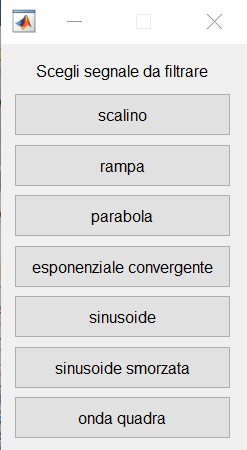
\includegraphics[scale=.7]{immaginiMain/mainfilterPOSS.png} 
\end{wrapfigure}
Una volta cliccato il pulsante \textit{Run} di matlab la prima schermata permette la scelta del segnale da filtrare.
A destra il layout di tale schermata con tutte le possibili scelte cliccabili.\\
Cliccando uno dei segnali il programma provvederà alla creazione del sistema relativo alla generazione di tale segnale.
\begin{lstlisting}[frame=single]
sys = ss(A,B,C,D);
sysd = c2d(sys,dt);
[Ad,Bd,Cd,Dd] = ssdata(sysd);
\end{lstlisting}
Successivamente viene assegnata la matrice di covarianza del rumore di processo :
\begin{lstlisting}[frame=single]
Q = 1e-5;
\end{lstlisting}
A questo punto si procede alla generazione dell'oggetto della classe kalmanfilter, che verrà utilizzato per la stima e il filtraggio del segnale, utilizzando le matrici relative alla discretizzazione del modello precedente e lo stato 0 come stato iniziale.
\begin{lstlisting}[frame=single]
k=kalmanfilter(Ad,Bd,Cd,Dd,Q,R,x0,P0);
\end{lstlisting}

A questo punto il programma procede con il calcolo dell'evoluzione dello stato e con il plottaggio e l'animazione della stima effettuata dal filtro, il tempo dell'animazione, e la variazione delle matrici di  covarianza dello stato e del guadagno.\\
Di seguito viene riportato un esempio del filtraggio di uno scalino affetto da rumore :


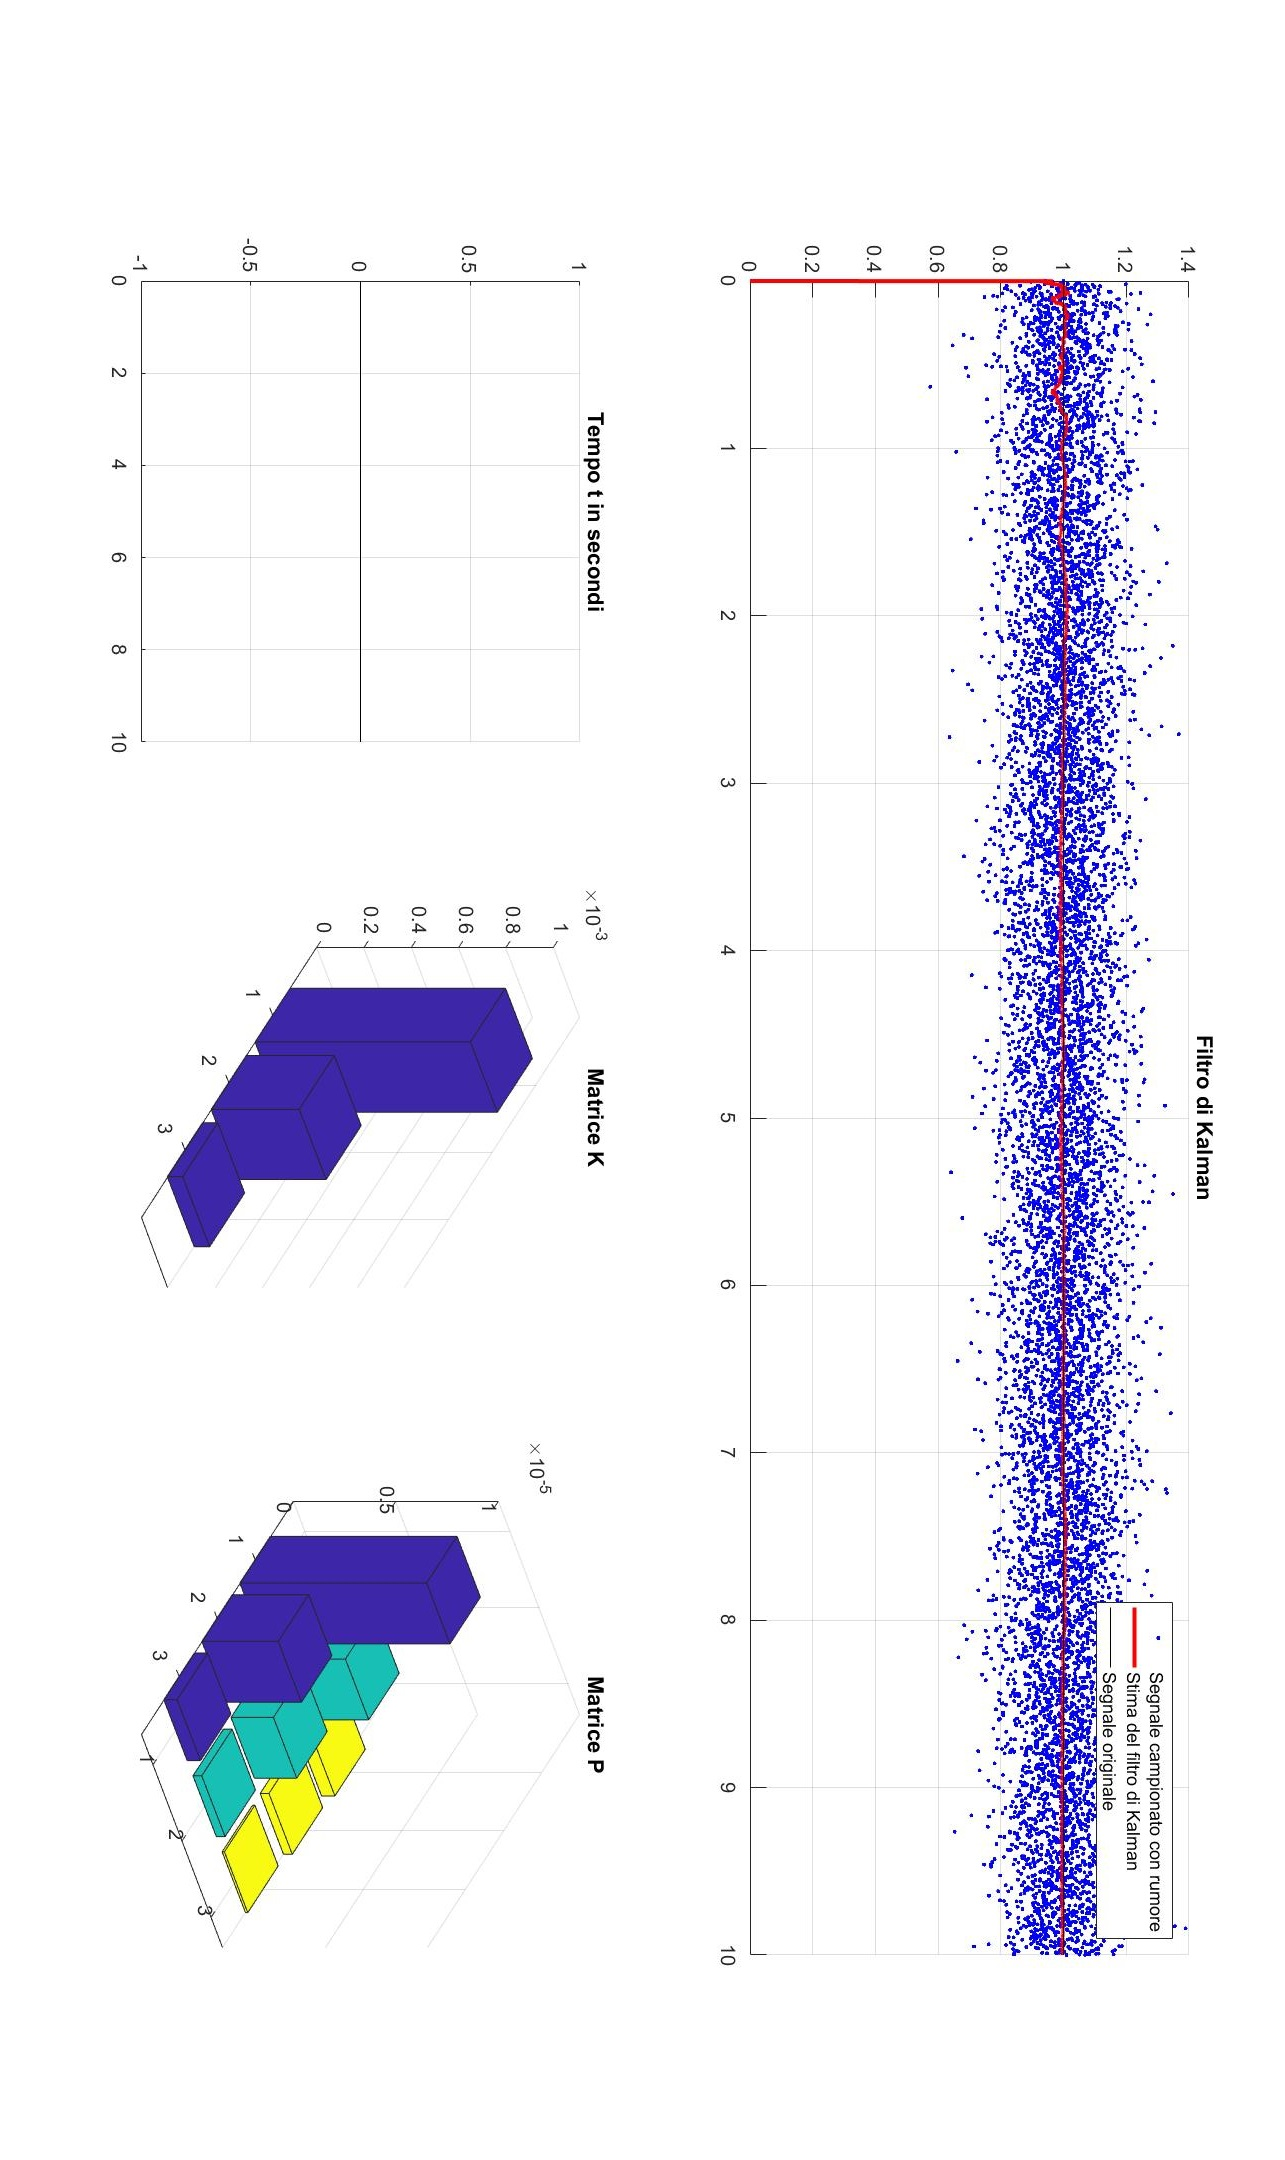
\includegraphics[scale=.5]{immaginiMain/esempio.jpg} 




\newpage